\documentclass{report}
\usepackage[T1]{fontenc} % Fontes T1
\usepackage[utf8]{inputenc} % Input UTF8
\usepackage[backend=biber, style=ieee]{biblatex} % para usar bibliografia
\usepackage{csquotes}
\usepackage[portuguese]{babel} %Usar língua portuguesa
\usepackage{blindtext} % Gerar texto automaticamente
\usepackage[printonlyused]{acronym}
\usepackage{hyperref} % para autoref
\usepackage{graphicx}
\usepackage{hyperref}

\bibliography{bibliografia}


\begin{document}
%%
% Definições
%
\def\titulo{\textbf{Projeto 2}}
\def\data{15 de Junho de 2019}
\def\autores{Vasco Sousa, Miguel Cabral,\\ Tiago Rainho, Francisco Monteiro}
\def\autorescontactos{(93049) jvcs@ua.pt, (93091) miguel.f.cabral@ua.pt,\\ (92984) tiago.rainho@ua.pt, (93105) francisco.monteiro@ua.pt}

\def\departamento{Departamento de Eletrónica, Telecomunicações e Informática}
\def\empresa{\ac{ua}}
\def\logotipo{ua.pdf}
\def\codeua{\href{https://code.ua.pt/projects/labi2019-p2-g12}{CODEUA}}
%
%%%%%% CAPA %%%%%%
%
\begin{titlepage}

\begin{center}
%
\vspace*{50mm}
%
{\Huge \titulo}\\ 
%
\vspace{10mm}
%
{\Large \empresa}\\
%
\vspace{10mm}
%
{\LARGE \autores}\\ 
%
\vspace{30mm}
%
\begin{figure}[h]
\center
\includegraphics{\logotipo}
\end{figure}
%
\vspace{30mm}
\end{center}
%
\begin{flushright}

\end{flushright}
\end{titlepage}

%%  Página de Título %%
\title{%
{\Huge\textbf{\titulo}}\\
{\Large \departamento\\ \empresa}
}
%
\author{%
    \autores \\
    \autorescontactos
}
%
\date{\data}
%

\maketitle

\pagenumbering{roman}

%%%%%% RESUMO %%%%%%
\begin{abstract}
O nosso projeto consiste numa aplicação web que recebe imagens, envia-as para um endereço que as analisa e devolve possíveis objetos detetados. É suportada por uma interface web que é muito simples de se trabalhar. Depois de enviada a imagem são recortadas as imagens dos objetos e armazenadas para futura pesquisa. A pesquisa pode ser feita através do nome do objeto detetado e também através da cor predominante. Podemos também alterar o nível de confiança de cada objeto entre 0 e 100, em que 0 mostrará todos os objetos detetados de acordo com a pesquisa e 100 só mostrará aqueles que o sistema detetou com 100\% de certeza do que eram. O código é feito maioritariamente em python, mas também utilizámos o Sqlite3 para criar a base de dados. Já a interface web utiliza \ac{html}, \ac{css}, \ac{js} e também Bootstrap.

\end{abstract}

%%%%%% Agradecimentos %%%%%%
\renewcommand{\abstractname}{Agradecimentos}
\begin{abstract}
Queremos agradecer a todos os docentes que lecionam a  \ac{uc} de \ac{labi} que no conjunto destes dois semestres nos deram os conhecimentos para a realização deste projeto.
\end{abstract}


\tableofcontents
% \listoftables
\listoffigures    


%%%%%%%%%%%%%%%%%%%%%%%%%%%%%%%
\clearpage
\pagenumbering{arabic}

%%%%%%%%%%%%%%%%%%%%%%%%%%%%%%%%
\chapter{Introdução}
\label{chap.introducao}

Este relatório foi elaborado com o propósito de descrever e analisar o segundo projeto realizado no âmbito da \ac{uc} de \ac{labi}.

Este documento está dividido em oito capítulos.
Depois desta introdução,
 é apresentada a metodologia seguida,
no \autoref{chap.interface web} é apresentada a interface web do sistema, no \autoref{chap.aplicacaoweb} é explicitado todo o código python desenvolvido no sistema, na \autoref{chap.persistencia} é abordada a base de dados. No \autoref{chap.processador} é abordado o funcionamento do processador de imagens.No \autoref{chap.resultados} são explicitados os resultados e no \autoref{chap.analise} é feita a análise destes resultados.
Finalmente, no \autoref{chap.conclusao} são apresentadas
as conclusões do trabalho.

\chapter{Interface web}
\label{chap.interface web}
Esta componente é composta por 5 páginas desenvolvidas através de  \ac{html}, \ac{js} e \ac{css} fornecendo a interface para a interação com o sistema. A aplicação web é simples e fácil de entender para qualquer utilizador, pelo que foi desenhada para ser fácil de trabalhar, funcional e organzada.

\section{HTML, CSS e Javascript}
Neste projeto, utilizámos estes recursos como é normal na criação de websites. O ac{html} é a principal base da aplicação web, sendo que é onde se implementam as várias divisões da aplicação. No ac{css} é onde se implementam os estilos das letras e das imagens. Isto ajuda a simplificar e a tornar apelativa a aplicação. O ac{js} ajuda a implementar certas funcionalidades e dinâmicas na interface web. Este ajuda a tornar a página mais interativa para o utilizador. Estes são os principais aspetos da interface web. Utilizámos também o Bootstrap para nos ajudar a tornar a página mais simples e interativa para o utilizador.

\section{Funcionalidades de cada página web}
A interface web está dividida em cinco páginas distintas. A primeira página da interface web é composta pela listagem de todos os objetos detetados nas imagens enviadas e a quantidade de vezes que já foi detetado.\par Na segunda página, é implementada a funcionalidade de procura de imagens pelo nome. As imagens que aparecem são as que foram detetadas e recortadas. Pode também ajustar o nível de confiança de deteção, entre 0 e 100, sendo que predefinidamente estará a 50. \par Na terceira página, é onde pode enviar novas imagens para o sistema, para a sua deteção. \par Na quarta, irá restringir a pesquisa, pois é possível pesquisar por nome e por cor. As únicas cores disponíveis são o vermelho, o verde e o azul, visto que estamos a utilizar o modo de cores RGB. Assim, as imagens que aparecerão nesta página, serão as que tiverem predominantemente a cor escolhida para pesquisa. \par Já a quinta página, é apenas abordada a informação sobre os autores do projeto.

\section{Responsividade}
A aplicação web tem várias caraterísticas. Uma delas é a responsividade, isto é, é possível visualizar a aplicação em qualquer dispositivo de qualquer tamanho sem alterar a integridade da mesma. Utilizámos também uma \textit{navbar} para facilitar a mudança de funcionalidade pelo utilizador, clicando na aba que quer utilizar.


\chapter{Aplicação Web}
\label{chap.aplicacaoweb}
A aplicação web é composta por um programa em python que apresenta métodos que permitem o fluxo de informação entre as diversas componentes.

\section{Lista de objetos}
A primeira página é composta por uma lista de todos os objetos já detetados, de todas as imagens inseridas. A listagem é conseguida através da chamada de \textbf{\textit{/list?type=names }} que devolve um objeto \ac{json} com um array de todos os objetos detetados no sistema. Por exemplo: 
\vspace{5 mm}
\begin{figure}[!ht]
    \centering
    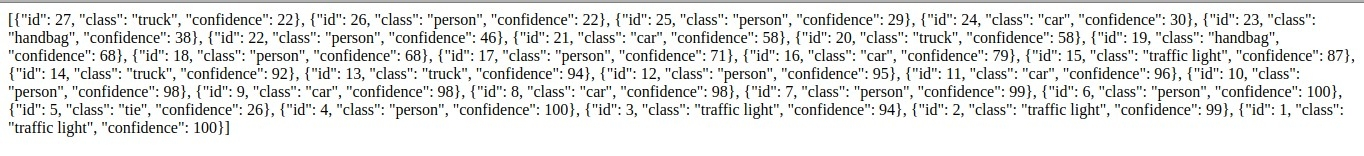
\includegraphics[scale = 0.3]{foto.jpg}
    \caption{Objeto \ac{json}}
    \label{fig:my_label}
\end{figure}

A função \textbf{\textit{/list?type=detected}} devolve um objeto JSON com uma lista das pequenas imagens contendo os objetos extraídos e o nível de confiança e a imagem original. O exemplo abaixo mostra isso :

\vspace{5 mm}
\begin{figure}[!ht]
    \centering
    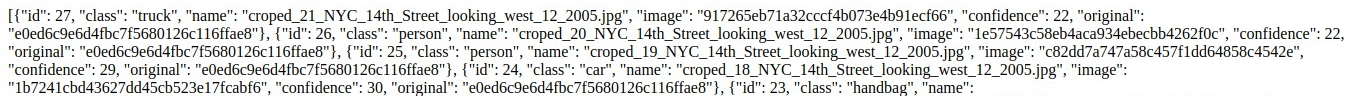
\includegraphics[scale = 0.3]{detect.jpg}
    \caption{Objeto \ac{json}}
    \label{fig:my_label}
\end{figure}

A função  \textbf{\textit{/list?type=detected\&name=NAME}} devolve um objeto \ac{json} com uma lista de pequenas imagens contendo os objetos extraídos que sejam relativos ao objeto referenciado pelo filtro NAME.
Por exemplo quando \textit{NAME} corresponde a \textit{person}:
\vspace{5 mm}
\begin{figure}[!ht]
    \centering
    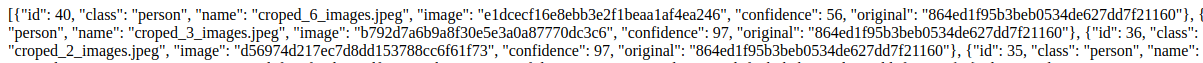
\includegraphics[scale = 0.3]{person.png}
    \caption{Objeto \ac{json}}
    \label{fig:my_label}
\end{figure}

A função  \textbf{\textit{/list?type=detected\&name=NAME\&color=COLOR}} devolve um objeto \ac{json} tem a mesma função que a anterior mas com um filtro adicional (COLOR).
Por exemplo quando \textit{COLOR} corresponde a \textit{green}:
\vspace{5 mm}
\begin{figure}[!ht]
    \centering
    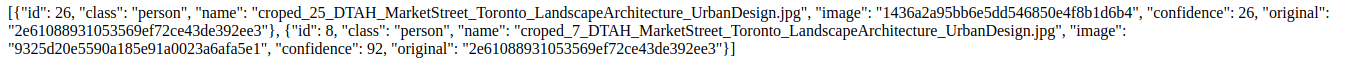
\includegraphics[scale = 0.3]{green.png}
    \caption{Objeto \ac{json}}
    \label{fig:my_label}
\end{figure}


\chapter{Persistência}
\label{chap.persistencia}
Para ajuda à regulação do armazenamento de imagens, criámos uma base de dados onde se encontra o caminho para as imagens. Desta forma, facilita a procura das imagens na pasta. Usámos o sqlite3 como linguagem para a base de dados. Nas imagens seguintes podemos visualizar o armazenamento do caminho para as imagens e a separação entre as imagens originais e as imagens recortadas. As imagens originais encontram-se na pasta original e as imagens recortadas encontram-se na pasta objects.

\begin{figure}[!ht]
    \centering
    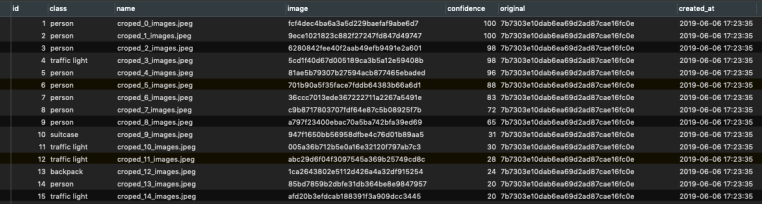
\includegraphics[scale = 0.5]{dbObjects.png}
    \caption{Tabela dos Objetos detetados}
    \label{fig:bdobjs}
\end{figure}

Na tabela anterior, podemos visualizar que há várias colunas, cada uma correspondente a uma caraterística das imagens. A coluna \textit{class} é referente ao objeto em si, por exemplo, uma pessoa. A coluna \textit{name} é o nome do ficheiro da imagem. A coluna \textit{image} é a encriptação do nome do ficheiro da imagem recortada e a \textit{original} é a encriptação do nome do ficheiro da imagem original. A coluna \textit{confidence} é referente à confiança da imagem, em que quanto maior a confiança, maior a certeza de que a imagem é o objeto indicado, da cor indicada e a última coluna é a data em que a imagem foi enviada.


\begin{figure}[!ht]
    \centering
    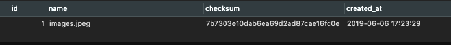
\includegraphics[scale = 0.7]{dbImagens.png}
    \caption{Tabela das Imagens Enviadas}
    \label{fig:bdimages}
\end{figure}

Nesta tabela, podemos visualizar as imagens enviadas, sendo que na primeira coluna temos o nome da imagem original e na coluna seguinte a sua encriptação. É aqui que ficam armazenadas as imagens originais enviadas pelo utilizador.

\chapter{Processador de Imagens}
\label{chap.processador}
Esta componente é o responsável pelo processamento das imagens. Fizémo-lo de modo a que a imagem seja enviada automaticamente para o endereço disponibilizado no enunciado do projeto, e que devolve um objeto ac{json} que é interpretado nesta componente. Utilizámos também o algoritmo fornecido pelos docentes da ac{uc} para enviar automaticamente as imagens para o tal endereço.

\chapter{Resultados}
\label{chap.resultados}
Com este projeto procurávamos executar tudo o que foi pedido no guião e torná-lo o mais simples possível para qualquer utilizador conseguir utilizar. Assim, o resultado foi positivo, pelo que conseguimos executar todas as tarefas pedidas de forma eficaz. Como conseguimos concluir tudo antecipadamente, decidimos também acrescentar outra funcionalidade, que é a remoção de objetos detetados que o sistema detetou. Assim, o utilizador pode apagar objetos que enviou e a sua imagem correspondente, simplesmente clicando no botão que está abaixo desse objeto.

\chapter{Análise}
\label{chap.analise}
A nossa análise aos resultados são que não podia ter corrido melhor, visto que cumprimos todos os requisitos pedidos no enunciado do projeto e ainda acrescentámos outra funcionalidade. Assim, simplesmente acrescentamos que não só concluímos tudo, como também deixámos tudo simples de perceber e para qualquer utilizador poder trabalhar.

\chapter{Conclusões}
\label{chap.conclusao}
Concluímos assim que este projeto foi um sucesso, pois concluímos todas as etapas pedidas. Conseguimos outro objetivo nosso que era deixar tudo simples e fácil de perceber e de trabalhar para o utilizador. Depois de tudo feito, ainda acrescentámos outra funcionalidade, pois achámos que poderíamos ainda melhorar o nosso projeto. Com isto, podemos concluir que acabámos o projeto da melhor maneira e que cumprimos todos os requisitos do enunciado do projeto, sem complicar a forma de usar a nossa interface web.

\chapter*{Contribuições dos autores}
O autor \ac{vs} fez um total de ...
O autor \ac{fm} fez um total de ...
O autor \ac{mc} fez um total de ...
O autor \ac{tr} fez um total de ...\\
\begin{center}\LARGE{
\href{https://code.ua.pt/projects/labi2019-p2-g12}{Code UA}
}\end{center}

\chapter*{Acrónimos}
\begin{acronym}
\acro{labi}[LABI]{Laboratórios de Informática}
\acro{ua}[UA]{Universidade de Aveiro}
\acro{uc}[UC]{Unidade Curricular}
\acro{html}[HTML]{Hyper Text Markup Language}
\acro{js}[JS]{JavaScript}
\acro{css}[CSS]{Cascading Style Sheets}
\acro{json}[JSON]{JavaScript Object Notation}
\acro{vs}[VS]{Vasco Sousa}
\acro{fm}[FM]{Francisco Monteiro}
\acro{mc}[MC]{Miguel Cabral}
\acro{tr}[TR]{Tiago Rainho}

\end{acronym}

\end{document}